%! Author = Ivan
%! Date = 2024-05-07
\documentclass[tikz]{standalone}
\usepackage{lib/basic}
\begin{document}
   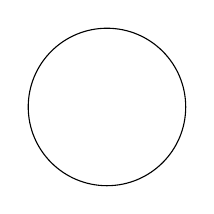
\begin{tikzpicture}[]
%    \def\pindist{35pt}
%    \def\nodesize{38pt}
%    \tikzstyle{every pin edge}=[signal]
%    \tikzstyle{annot} = [text width=4em, text centered]
%       \node[hiddennode, text width=\nodesize, minimum size=\nodesize,
%        pin={[pin edge={latex-}, pin distance=\pindist]above left:$x_1$},
%        pin={[pin edge={latex-}, pin distance=\pindist]below left:$x_2$},
%        pin={[pin edge={-latex}, pin distance=\pindist]right:$y_1$}
%        ] (N1) at (-100pt,0) {$f(x)$};
%     \node[hiddennode, text width=\nodesize, minimum size=\nodesize,
%        pin={[pin edge={-latex}, pin distance=\pindist]above left:$\frac{\partial L}{\partial x_1}=\frac{\partial L}{\partial y_1}\frac{\partial y_1}{\partial x_1}$},
%        pin={[pin edge={-latex}, pin distance=\pindist]below left:$\frac{\partial L}{\partial x_2}=\frac{\partial L}{\partial y_1}\frac{\partial y_1}{\partial x_2}$},
%        pin={[pin edge={latex-}, pin distance=\pindist]right:$\frac{\partial L}{\partial y_1}$}
%        ] (N2) at (+120pt,0) {$\diff f$};
%    \node[annot, text width=200pt, align=center, above=40pt of N1] (l1) {Forwardpass};
%    \node[annot, text width=200pt, align=center, above=40pt of N2] (l2) {Backwardpass};
%    \draw[signal, -] (0,-70pt) -- (0,+80pt);
       \draw (1,1) ellipse (1 and 1);
    \end{tikzpicture}
\end{document}